%!TEX root = index.tex
\section[Introdução]{Introdução}
\begin{frame}{Introdução}
O que são Sistemas de Recomendação?
\begin{block}{Definição}
``São ferramentas e técnicas de software destinadas a prover sugestões de itens para usuários'' \cite{ricci2011introduction-chap1}
\end{block}
\end{frame}

\begin{frame}{Introdução}{Aplicações}
\begin{columns}[c] % The "c" option specifies centered vertical alignment while the "t" option is used for top vertical alignment

\column{.5\textwidth} % Left column and width

\begin{figure}[ht]
    \begin{center}
    
\includegraphics[height=30px]{img/facebook}

    Relações de amizade
    \end{center}
\end{figure}

\begin{figure}[ht]
    \begin{center}
    \includegraphics[height=30px]{img/lastfm}

    Músicas
    \end{center}
\end{figure}

\column{.5\textwidth} % Right column and width

\begin{figure}[ht]
    \begin{center}
    
\includegraphics[height=30px]{img/amazon}

    Livros
    \end{center}
\end{figure}

\begin{figure}[ht]
    \begin{center}
    
\includegraphics[height=30px]{img/google-news}

    Notícias
    \end{center}
\end{figure}

\end{columns}
\end{frame}

\begin{frame}{Introdução}
\begin{figure}[ht]
    \begin{center}
    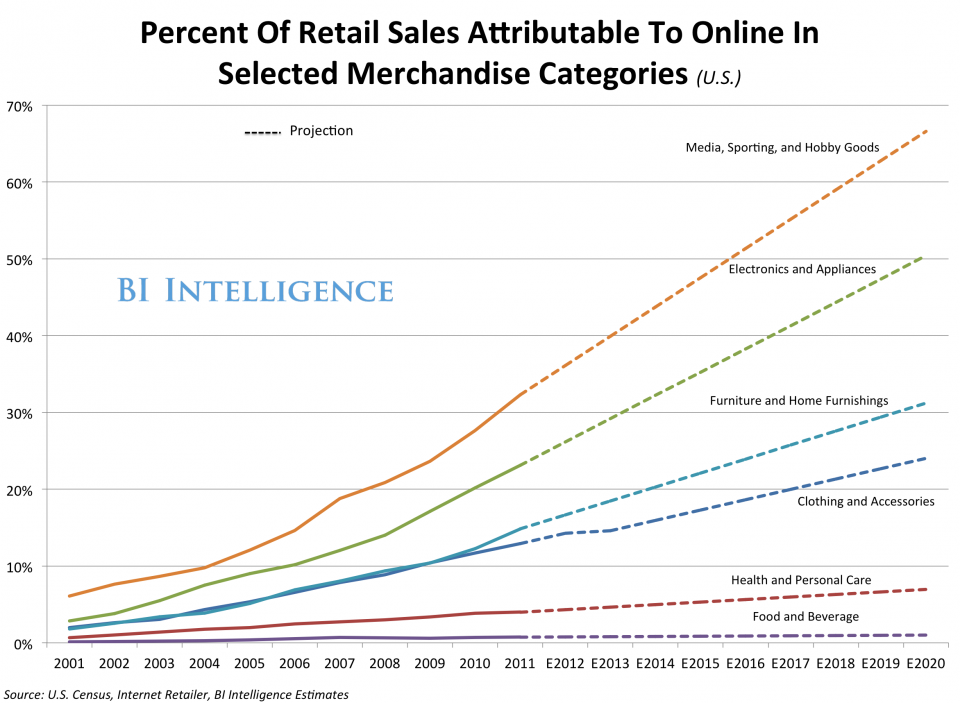
\includegraphics[width=0.8\textwidth]{img/crescimento-ecommerce}\caption{Percentual de vendas de varejo atribuídas a lojas online \cite{crescimento-ecommerce}}
    \end{center}
\end{figure}
\end{frame}

\begin{frame}{Introdução}
\begin{figure}[ht]
    \begin{center}
    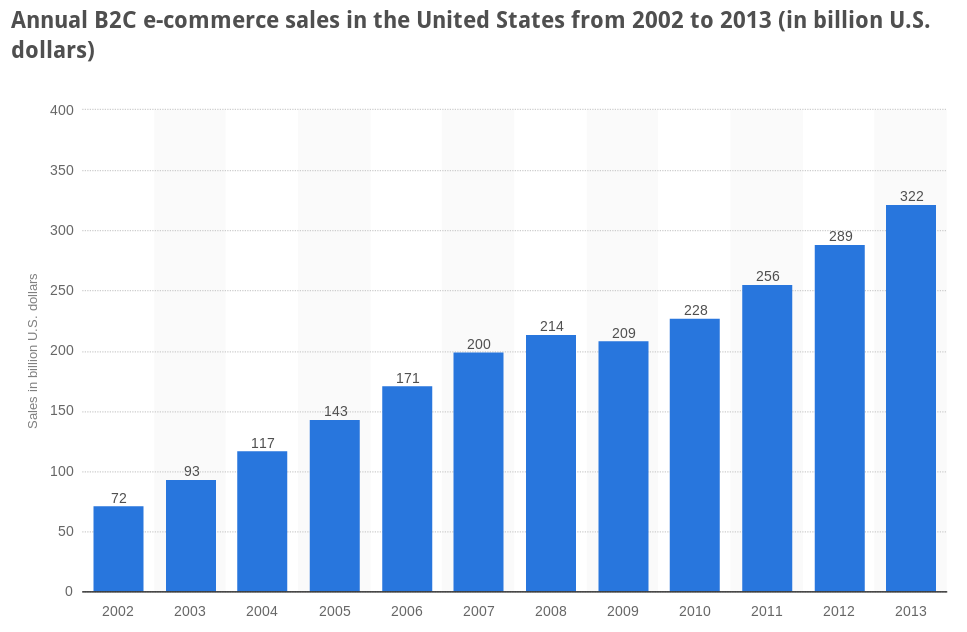
\includegraphics[width=0.8\textwidth]{img/sales-ecommerce}\caption{Vendas anuais em e-commerces nos EUA \cite{sales-ecommerce}}
    \end{center}
\end{figure}
\end{frame}

\begin{frame}
\frametitle{Introdução}
\begin{block}{Etapas principais}
\begin{itemize}
	\item Aquisição dos dados de entrada
	\item Determinação das recomendações
	\item Apresentação dos resultados ao usuário
\end{itemize}
\end{block}
\end{frame}

\begin{frame}
\frametitle{Introdução}
\begin{block}{Etapas principais}
\begin{itemize}
	\item Aquisição dos dados de entrada
	\item Determinação das recomendações
	\item Apresentação dos resultados ao usuário
\end{itemize}
\end{block}
\end{frame}

\begin{frame}
\frametitle{Introdução}
\begin{itemize}
	\item importância econômica de lojas online
	\item criação de ferramentas \textit{open source} para a comunidade
\end{itemize}

\begin{center}
$\Downarrow$ 
\end{center}

\begin{center}
Desenvolvimento de um sistema de recomendação \par{} de produtos para e-commerces
\end{center}

\end{frame}
